\documentclass[11pt,a4paper,French]{article}

\usepackage{subfiles}
\usepackage[utf8]{inputenc}
\usepackage[T1]{fontenc}
\usepackage[french]{babel}
\usepackage{graphicx}


\begin{document}
%Title Page of Hoar
\begin{center}
  \vspace*{1cm}
  \Huge \textbf{Tony Hoare}

  \Large{Un bref apercue}
  \vspace{0.8cm}

   \begin{minipage}{0.6\textwidth}
    \large \em{\hspace*{20mm}\flq{}There are two methods in

    software design. One is to make the program so simple,

     there are obviously no errors.}

    {The other is to make it so complicated,

    there are no obvious errors.\frq{}}
  \end{minipage}
  \begin{minipage}{0.3\textwidth}
    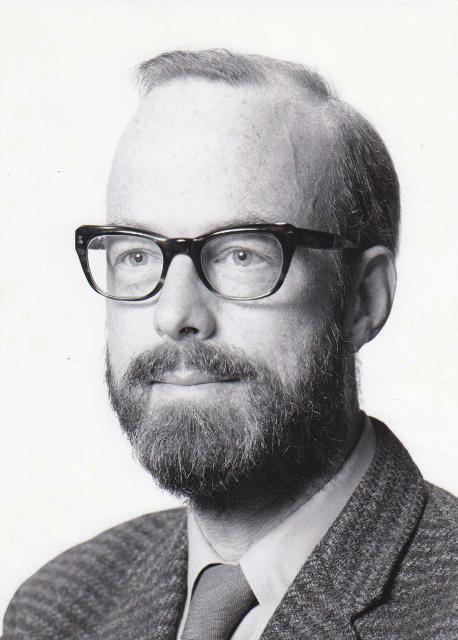
\includegraphics[width=\textwidth]{./img/PHoar.jpg}
  \end{minipage}
\end{center}
%End title Page of Hoar
  \tableofcontents
  \subfile{Intro}
  \subfile{logique}
  \subfile{quicksort}

\end{document}
